\documentclass[aspectratio=169,t,11pt,table]{beamer}
\usepackage{slides,math}
\definecolor{accent}{HTML}{940034}
\definecolor{accent2}{HTML}{006896}

\title{Simple Difference-in-Differences Estimation in Fixed-$T$ Panels}
\date{\today}
\author{Kyle Butts, Nicholas Brown, and Joakim Westerlund}
\addbibresource{references.bib}

\def\*#1{\mathbf{#1}}
\def\+#1{\boldsymbol{#1}}
\begin{document}

% ------------------------------------------------------------------------------
\begin{frame}[noframenumbering,plain]
  \maketitle
\end{frame}
% ------------------------------------------------------------------------------

% ------------------------------------------------------------------------------
\section{Motivation}
% ------------------------------------------------------------------------------

\begin{frame}{Motivation}
  Treatment is often targeted to places/units based on their economic trends:

  \begin{itemize}    
    \only<1->{
      \item New apartment construction \citep{asquith2021local,pennington2021does}
      \begin{itemize}
        \item Built in appreciating neighborhoods
      \end{itemize} 
    }

    \pause
    \item Walmart entry \citep{basker2005job,neumark2008effects}
    \begin{itemize}
      \item Open stores in areas with growing retail spending
    \end{itemize}

    \pause
    \item Place-based policies \citep{neumark2015place}
    \begin{itemize}
      \item Target places with declining labor markets 
    \end{itemize}
  \end{itemize}

  \bigskip\pause
  Standard difference-in-differences assumption of parallel trends is \emph{implausible}
\end{frame}


\begin{frame}{Motivation}
  In some settings, the causes of these trends are due to larger economic forces and not location-specific shocks:
  
  \begin{itemize}
    \item New apartment construction
    \begin{itemize}
      \item Changing preferences for walkable neighborhoods
    \end{itemize} 

    \pause
    \item Walmart entry
    \begin{itemize}
      \item Growing employment increases disposable income
    \end{itemize}

    \pause
    \item Place-based policies
    \begin{itemize}
      \item Decline of manufacturing hurting manufacturing hubs
    \end{itemize}
  \end{itemize}
\end{frame}

\begin{frame}{Modeling differential trends}
  This paper models differential trends using a \textbf{factor model} that is popular in the finance/macroeconomics literature:

  \begin{itemize}
    \item Each time period there is a set of \emph{unobservable} \textbf{macroeconomic/regional shocks} that are common across units
    \item Units vary based on their \emph{unobservable} baseline characteristics in how impacted they are by the shocks
  \end{itemize} 
\end{frame}

\begin{frame}{Empirical Approach}
  This paper proposes to control for these confounding shocks by using a set of \textbf{auxiliary covariates} that are impacted by the \textbf{same} set of macroeconomic shocks that affect the outcome variable

  \begin{itemize}
    \item The idea is to use the covariates to \emph{`reveal'} to us the confounding shocks over time and then control for them 
  \end{itemize}

  \bigskip
  Controlling for the confounding shocks allows us to isolate the treatment effect
\end{frame}

\begin{frame}{Contribution}{Using covariates to inform us about confounders}
  Similar to us, \citet{freyaldenhoven2019pre} propose a method of using a covariate $x_{it}$ that is informative about the confounding shock to $y_{it}$.
  
  \bigskip
  Relative to their paper,
  \begin{itemize}
    \item Our estimator is treatment effect heterogeneity robust
    
    \item We allow for treatment to (potentially) impact the value of the covariate $x_{it}$
  \end{itemize}
\end{frame}

\begin{frame}{Contribution}{Time-varying covariates in Difference-in-differences}
  There is a dilemma about using time-varying covariates in DID \citep{Caetano_Callaway_Payne_Rodrigues_2022}:

  \begin{itemize}
    \item Parallel trends type assumptions often times rely on conditioning on a set of \emph{time-varying} covariates, $\*x$

    \item However, if treatment impacts the value of $\*x$, then controlling for their post-treatment value absorbs treatment effect
    \begin{itemize}
      \item \citet{angrist2009mostly} call this a ``bad control''
    \end{itemize}
  \end{itemize}
\end{frame}

\begin{frame}{Contribution}{Time-varying covariates in Difference-in-differences}
  For example, consider estimating the effect of a certain policy aimed at reducing unemployment
  \begin{itemize}
    \item We might want to control for the rate of poverty to address possible confounding
    
    \item Such policies might indirectly reduce poverty, which means that the poverty rate covariate will absorb some of the treatment effect.
  \end{itemize}

  \pause
  \bigskip 
  We solve this by predicting what $\*x$ would have been in the absence of treatment and control for that
  \begin{itemize}
    \item We also show how to estimate the `mediated' effect that operates through changes to $\*x$
  \end{itemize}
\end{frame}

% ------------------------------------------------------------------------------
\section{Setup}
% ------------------------------------------------------------------------------

\begin{frame}{Outcome model}
  There are $i \in \{ 1, \dots, N \}$ units and $t \in \{ 1, \dots, T \}$ time periods. 
  \begin{itemize}
    \item Treatment turns on in period $T_0 + 1$.
    \item $D_i$ is a dummy varaible denoting treated units and $d_{it}$ be a dummy when treatment is \emph{active}
  \end{itemize}
  
  \bigskip
  Untreated potential outcomes are modeled as
  $$
    y_{it}(0) = \*x_{it}\beta + \sum_{r = 1}^{p} \orange{\gamma_{i,r}} * \purple{f_{t,r}} + u_{it}
  $$

  \begin{itemize}
    \item $f_{t, r}$ is the $r$-th \textbf{\color{purple} factor} (macroeconomic shock) at time $t$.
    \item $\gamma_{i,r}$ is unit i's \textbf{\color{orange} factor loading} (exposure) to the $r$-th factor.
  \end{itemize}
\end{frame}

\begin{frame}{Covariates are impacted by same shocks}
  The intuition of our approach is that we have a set of $K$ covariates that are impacted by the same set of shocks that impact the outcome.
  
  \medskip
  Formally, the $K$ observed covariates $\* x_{it}$ are generated as follows:
  \begin{align}
    x_{k,it}(0) = \+\lambda_{i,k}'\*f_t + v_{k,it},
  \end{align}
  with $\*v$ is mean zero vector of errors.

  \begin{itemize}
    \item We allow for the possibility that treatment impacts some of the elements of $\*x$!

    \item $\*x$ can not be time-invariant.
  \end{itemize}
\end{frame}

\begin{frame}{Estimand}
  Our goal is to estimate event-study style estimators:
  $$
    \expec{y_{t}(1) - y_{t}(0)}{D = 1}
  $$

  We follow a new approach and `impute' $y_{it}(0)$ for the post-treatment observations to estimate these treatment effects \citep{borusyak2021revisiting,brown2022generalized}
\end{frame}

\begin{frame}{Common-Correlated Effects Approach}
  For a given $t$, taking the cross-sectional average of $x_{k,it}$ for the never-treated units ($D_i = 0$) gives us 
  \begin{align*}
    \expec{\*x_{it}}{D_i = 0} &= \expec{\+\lambda_{i,k}}{D_i = 0}' \* f_t + \expec{v_{k,it}}{D_i = 0} \\
    &= \expec{\+\lambda_{i,k}}{D_i = 0}' \* f_t \equiv \hat{\* f}_t
  \end{align*}

  Stacking these for all $t$ gives 
  $$ 
    \hat{\* F} = \expec{\+\lambda_{i,k}}{D_i = 0}' \*F
  $$

  \begin{itemize}
    \item Gives us a (\emph{rotated}) estimate for the macroeconomic shocks
  \end{itemize}
\end{frame}

\begin{frame}{Estimating $\*\beta$}
  Using the untreated and not-yet-treated group $d_{it} = 0$, we can estimate $\hat{\beta}$ and $\hat{\*a}_i$ via OLS:
  $$
    y_{it} = \*x_{it} \*\beta + \*a_i' \hat{\* f}_t + u_{it}
  $$
  
  \bigskip
  Now we can proceed to imputation for the post-treatment outcomes!
\end{frame}

\begin{frame}{Imputation Procedure}{Covariates}
  For the post-treatment observations, we need to know what $\*x$ would have been without treatment. We can impute untreated potential outcomes for the covariates via:
  $$
    \hat{\*x}_{it}(0) = \hat{\*f_t} (\hat{\*F}_{t<T_0}'\hat{\*F}_{t<T_0})^{-1} \hat{\*F}_{t<T_0}' \*x_{i, t<T_0}
  $$

  \begin{itemize}
    \item Estimate what the covariate 
  \end{itemize}
\end{frame}

\begin{frame}{Imputation Procedure}{Outcome}
  At last, we can impute the untreated potential outcomes for the post-treatment observations using:
  $$
    \hat{y}_{it}(0) = \hat{\*x}_{it}\hat{\*\beta} + \hat{\*a}_i' \hat{\*f}_t
  $$

  \bigskip
  \begin{itemize}
    \item The paper has all the econometric details on asymptotics and regularity conditions
  \end{itemize}
\end{frame}

\begin{frame}{Mediated effects}
  We can decompose the treatment effect into a portion that operatres through a `mediated effect',
  $$
    \expec{\*x_{it}\beta - \hat{\*x}_{it}(0)\beta}{D_i = 1},
  $$
  and the remaining portion which the mediation literature calls the `direct effect'
\end{frame}


% ------------------------------------------------------------------------------
\section{Empirical Application}
% ------------------------------------------------------------------------------

\begin{frame}{Pro-competitive Effects of Trade Competition}
  We revisit \citet{lu2015trade}'s analysis of China's accession into the World Trade Organization (WTO) in the end of 2001 to estimate the pro-competitive impacts of trade

  \bigskip
  Using values prior to WTO asscension, the authors compare industries with above-median tariffs (treated) to industries with below-median tariffs 
  \begin{itemize}
    \item Industries with larger tariffs prior to asscension, have larger increases in import competition
  \end{itemize}
\end{frame}

\begin{frame}{Variables of Interest}
  Using microdata on firms within industry, they estimate total factor productivity (TFP) and markups
  \begin{itemize}
    \item To summarize at the industry level, they calculate a `Theil index' which is a measure of the `dispersion' of the variable
  \end{itemize}

  \bigskip
  Intuitively, increasing import competition should decrease the dispersion of markups.
\end{frame}

\begin{frame}{Estimation of Treatment Effect}
  In our previous notation, $y_{it}$ is the Theil index of markup and $\*x_{it}$ is the Theil index of TFP. 
  \begin{itemize}
    \item Macroeconomic shocks that impact markups also likely to impact TFP 
    \item However, import competition might impact TFP (mediator)
  \end{itemize} 
  
  \bigskip
  Cross-sectional averages of $\*x_{it}$ and a constant are used to estimate $\hat{\*{F}}$ to add time fixed-effects. 
\end{frame}

\begin{frame}
  \begin{figure}
    \caption{Impact of China's WTO Asscension on Markup Dispersion}
    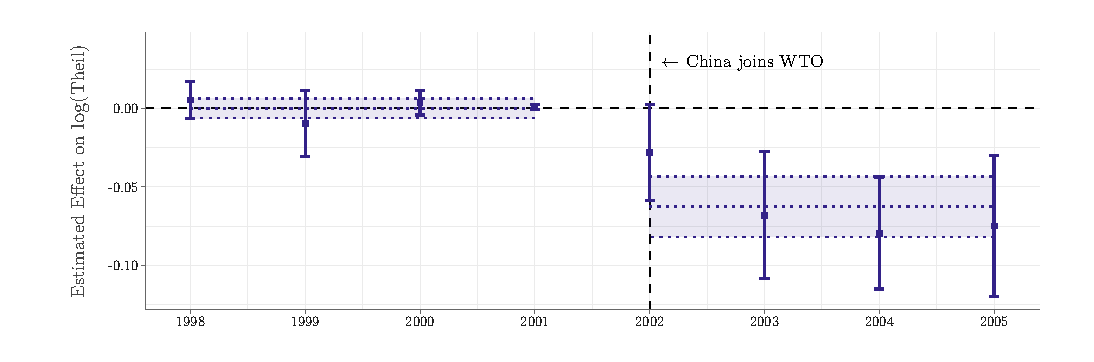
\includegraphics[width=\textwidth]{../../figures/trade-cce_est_interpolated.pdf}
  \end{figure}
\end{frame}

\begin{frame}{Mediated effects}
  \citet{lu2015trade} try to informally understand if markup dispersion declines are mediated via TFP dispersion declines
  \begin{itemize}
    \item They control for TFP dispersion in their TWFE model 
    \item The estimated treatment effect decreases, so they claim that `part of the effect' is driven by TFP dispersion declines
  \end{itemize}

  \bigskip
  This feels unsatisfactory and we want to say \emph{how much of the decline} is via TFP dispersion.
\end{frame}

\begin{frame}{Insights for time-varying covariates}
  As we discussed in the introduction and in \citet{Caetano_Callaway_Payne_Rodrigues_2022}, there is a dilemma with using time-varying covariates:
  \begin{itemize}
    \item time-varying covariates can be important for controlling for time-varying confounders
    
    \item However, if treatment affects these covariates, controlling for them will absorb some of the treatment effect
  \end{itemize}
\end{frame}

\begin{frame}
  \begin{figure}
    \caption{Mediated Effect via A Decline in TFP Dispersion}
    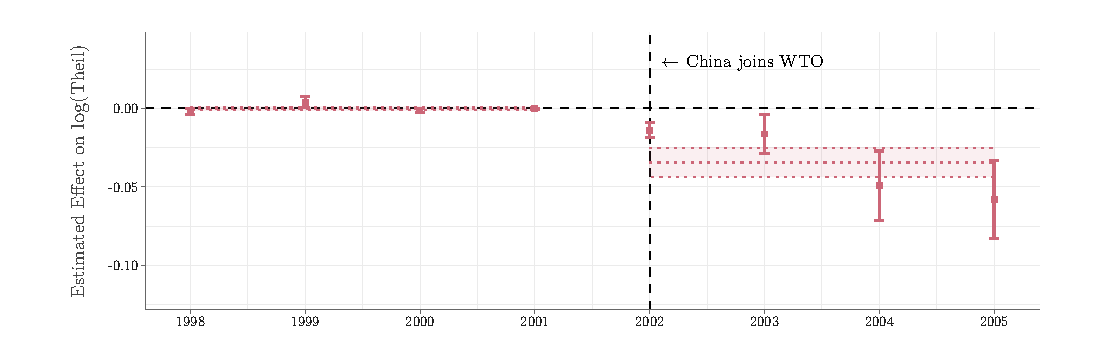
\includegraphics[width=\textwidth]{../../figures/trade-cce_mediated_est_interpolated.pdf}
  \end{figure}
\end{frame}

\begin{frame}
  \begin{figure}
    \caption{Problem with using observed $\*x_{it}$}
    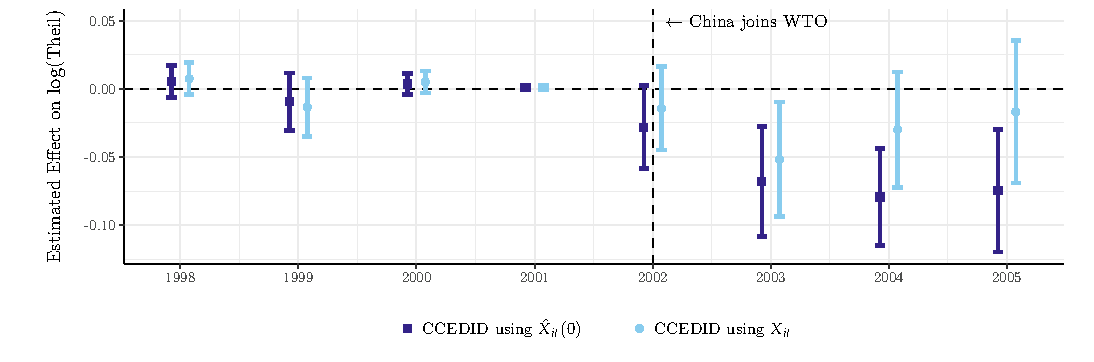
\includegraphics[width=\textwidth]{../../figures/trade-x0-vs-obs-x_interpolated.pdf}
  \end{figure}
\end{frame}

\begin{frame}{Conclusion}
  We bring the \emph{Common Correlated Effects} estimator into the realm of causal inference
  \begin{itemize}
    \item Covariates that inform us about confounding macroeconomic shocks can be used to `purge' this bias
  \end{itemize}

  \bigskip
  We allow for covariates to be impacted by treatment and decompose the treatment effect into a `direct effect' and a `mediated effect'
\end{frame}




% ------------------------------------------------------------------------------
\begin{frame}[allowframebreaks,noframenumbering]{References}
  \thispagestyle{empty}
  \printbibliography
\end{frame}
% \appendix
% ------------------------------------------------------------------------------


\end{document}
